\chapter{O teto do que se aprende}\label{cap:teto}

O capítulo da tolerância contou duas explicações de cento e oitenta, e o número ficou impresso como
se fosse uma propriedade do dado. Ele não é: é o \textbf{máximo} de uma família, e um máximo depende de
duas coisas que ninguém declarou --- quantas peças foram tentadas e quantos dias foram vistos. Este
capítulo varia as duas.

\section{A contagem é um máximo}

A peça que cabe é a que passa nas quatro tolerâncias ao mesmo tempo, e o que se conta é quantas
passam. Isso é um máximo sobre as tentativas: quanto mais peças se experimenta, mais fácil é que
alguma passe por acaso. E quanto mais dias se vê, mais difícil fica.

A conta do acaso é simples o bastante para ser dita. Se cada peça passa nas quatro provas com
chance $p$, independente das outras, então:

\begin{proposicao}[o teto das tentativas]\label{prop:teto-tentativas}
A chance de que ao menos uma peça da família passe é $1-(1-p)^{m}$, que cresce com o número de
peças tentadas $m$ e tende a um. E o número esperado de peças que passam é $mp$, de modo que
\textbf{a contagem mede $m$ e $p$ juntos}, e não o que o dado sabe.
\end{proposicao}

\begin{proof}
As $m$ peças são independentes com a mesma chance $p$ de passar, de modo que a chance de nenhuma
passar é $(1-p)^{m}$ --- e o complemento é o que a proposição afirma. O número esperado de sucessos
é $mp$ pela linearidade da esperança, que não precisa de independência. Como $1-(1-p)^{m}$ cresce em
$m$ para todo $p$ no intervalo, o teto sobe com o número de tentativas.
\end{proof}

A proposição não diz que as peças são de fato independentes --- não são, e o capítulo da bateria já
mediu o quanto isso pesa. Ela diz o que a contagem carrega: um fator $m$ que o leitor não vê.

\section{Medindo as duas coisas}

A família do capítulo da tolerância tem \numTetoPecasMaior{} peças na grade cheia e
\numTetoPecasMenor{} na grade mais grossa, e a série tem seis mil setecentos e dezoito dias. Variando
as duas coisas separadamente --- a grade por um lado, o comprimento da série por outro ---, a
contagem sai assim.

\begin{table}[htbp]\  \centering
  \small
  \begin{tabular}{lrrr}
    \hline
    peças tentadas & \numTetoDiasMenor{} dias & \numTetoDiasMeio{} dias & \numTetoDiasMaior{} dias \\
    \hline
    \numTetoPecasMenor & \numTetoDoisQuinhentos & \numTetoDoisDoisMil & \numTetoDoisSeisMilSetecentosEDezoito \\
    \numTetoPecasMeio & \numTetoTresQuinhentos & \numTetoTresDoisMil & \numTetoTresSeisMilSetecentosEDezoito \\
    \numTetoPecasMaior & \numTetoSeisQuinhentos & \numTetoSeisDoisMil & \numTetoSeisSeisMilSetecentosEDezoito \\
    \hline
  \end{tabular}
  \caption{As explicações que cabem na mesma tolerância, contra o tamanho da família e o número de
    dias vistos. A série é a do primeiro mercado, truncada. As três linhas são as três curvas do
    caderno, e a do meio é a que cruza a de cima no extremo longo.}
  \label{tab:teto}
\end{table}

Nas duas direções o número se move, e é isso que o capítulo da tolerância não dizia. Com a série
inteira e a grade cheia, cabem as duas de sempre. Com quinhentos dias e a mesma grade cheia, cabem
\numTetoSeisQuinhentos{} --- quase dez vezes mais, e nenhuma peça nova foi inventada: o que mudou
foi quanto se viu. E com a grade grossa e quinhentos dias, cabem \numTetoDoisQuinhentos{} das \numTetoPecasMenor{} peças --- uma em cada oito,
num dado que tem quinhentos dias.

E a ordem das famílias não se sustenta no extremo longo: com a série inteira, a grade de
\numTetoPecasMeio{} peças devolve \numTetoTresSeisMilSetecentosEDezoito{} onde a de
\numTetoPecasMaior{} devolve \numTetoSeisSeisMilSetecentosEDezoito{}. O cruzamento é do desenho
de um sorteio só, e nada nele diz que a família menor aprende mais --- diz que a contagem, com o
dado inteiro, já está na casa do que o sorteio sozinho mexe.

\begin{figure}[htbp]
  \centering
  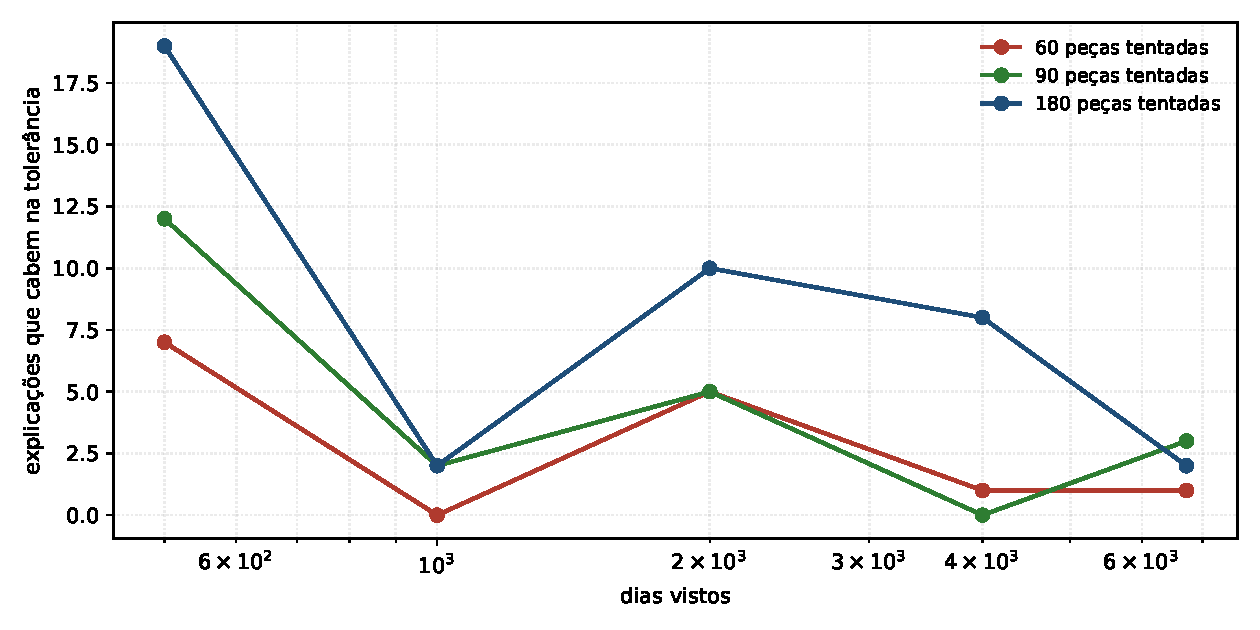
\includegraphics[width=\linewidth]{figuras/E28_teto_1.pdf}
  \caption{As explicações que cabem, contra os dias vistos, uma curva por tamanho de família. O eixo
    dos dias é logarítmico. A queda é a tendência, e não a regra: entre mil e quatro mil dias as
    curvas sobem e descem, e no extremo longo a família de \numTetoPecasMeio{} peças passa a de
    \numTetoPecasMaior{} --- \numTetoTresSeisMilSetecentosEDezoito{} contra
    \numTetoSeisSeisMilSetecentosEDezoito{}.}
  \label{fig:teto}
\end{figure}

\section{O outro teto: os bits}
% aterramento: esboco
% aterramento: contador
% aterramento: energia
% aterramento: precisao
% aterramento: contadores

O corte do capítulo da medida é contado com \textbf{um número por dia} --- são \numSerieDias{} deles ---,
e o pior bloco de sessenta dias é a leitura que destrava as voltas seguintes. Guardar cem números no
lugar de todos é o gesto mais natural do mundo. Este pedaço cobra o preço, e o preço não é o que se
imagina: não está no erro, está na pergunta.

Um contador não guarda dia nenhum: guarda uma \textbf{soma}. Some-se o fluxo inteiro a ele, cada
item com um sinal sorteado, e o que sobra é um número que sozinho não quer dizer nada. O quadrado
dele, em média sobre muitos sorteios, é que diz a \textbf{energia} do caminho --- a soma dos
quadrados dos incrementos, que é o segundo momento do fluxo.

\begin{proposicao}[o preço do resumo]\label{prop:preco-do-resumo}
Seja $Q = \sum_t r_t^2$ a energia do fluxo e sejam $K$ contadores $u_j$, cada um somando o fluxo
inteiro com sinais sorteados independentes. Então $\hat Q = \frac{1}{K}\sum_j u_j^2$ estima $Q$ sem
viés, com desvio relativo de no máximo $\sqrt{2/K}$. A precisão $\varepsilon$ custa, portanto,
$K = 2/\varepsilon^2$ contadores --- e nenhum método compra mais com menos.
\end{proposicao}

\begin{proof}
Cada $u_j$ é a soma $\sum_t \pm r_t$, com os sinais independentes, de média zero e variância um.
Os produtos de sinais distintos têm esperança zero, de modo que $\E[u_j^2] = \sum_t r_t^2 = Q$ --- e
é essa a conta inteira. A média sobre os contadores herda a esperança, e o estimador não tem viés.
Para o desvio, $\E[u_j^4] = 3Q^2 - 2\sum_t r_t^4$, de modo que a variância de $u_j^2$ é
$2Q^2 - 2\sum_t r_t^4$, que não passa de $2Q^2$. A média de $K$ contadores independentes divide
essa variância por $K$, e a raiz da razão entre as duas dá o desvio relativo.
\end{proof}

O limite é do problema, e não do estimador: estimar o segundo momento com erro relativo
$\varepsilon$ exige memória da ordem de $1/\varepsilon^2$, e esboço nenhum escapa disso
\cite{alon1999space}; o que se faz com $K$ contadores é ótimo até constante \cite{indyk2005optimal},
e cada outro momento tem o seu preço \cite{woodruff2004optimal}.

E esse teto matemático tem chão físico. O contador mora em matéria, e apagar um bit --- zerar a conta para a medição seguinte --- custa no mínimo $kT\ln 2$ de calor \cite{landauer1961irreversibility}: guardar e apagar o resumo é trabalho, e o mínimo desse trabalho é lei da termodinâmica, não do cálculo.

\begin{figure}[htbp]
  \centering
  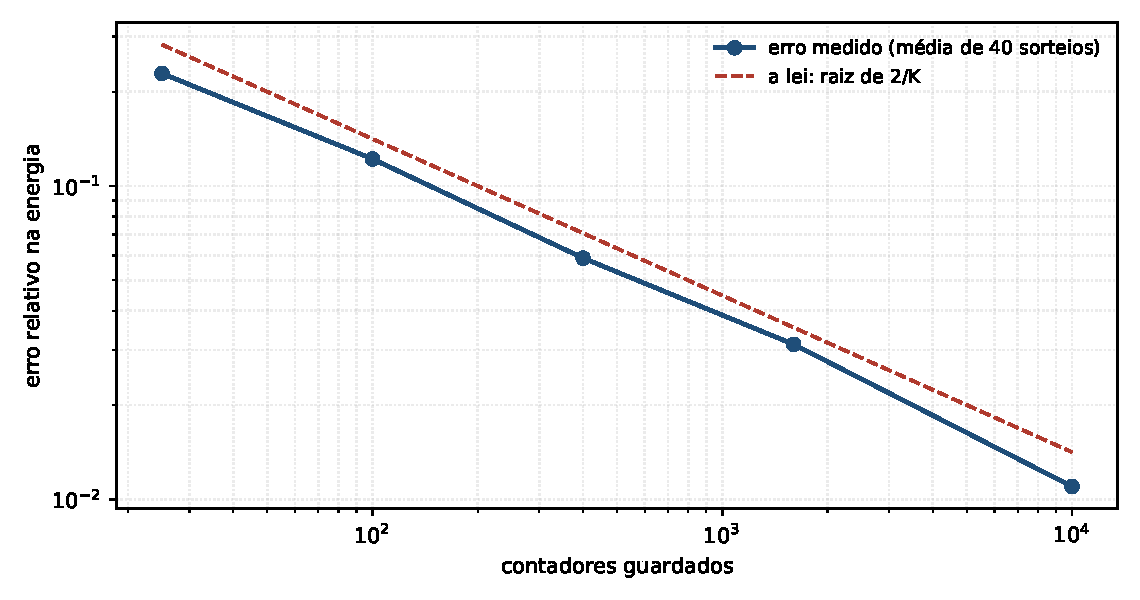
\includegraphics[width=\linewidth]{figuras/E29_bits_1.pdf}
  \caption{O erro do esboço contra o número de contadores guardados, nas duas escalas
    logarítmicas, com a reta da lei ao lado. As duas linhas são \textbf{paralelas}, e a medida
    fica abaixo da lei em toda a extensão: a média de uma estimativa simétrica custa cerca de
    oito décimos do desvio dela, e é isso que a distância entre as duas linhas mede.}
  \label{fig:bits}
\end{figure}

A medição usa o caminho do primeiro mercado --- os mesmos \numSerieDias{} dias, um número cada --- e
sorteia \numBitsMundos{} esboços por linha. O erro é o relativo na energia.

\begin{table}[htbp]
  \centering
  \small
  \begin{tabular}{rrr}
    \hline
    contadores guardados & erro medido (\%) & a lei prevê (\%) \\
    \hline
    \numBitsContadoresMenor & \numBitsErroVinteECinco & \numBitsPrevistoVinteECinco \\
    \numBitsCem & \numBitsErroCem & \numBitsPrevistoCem \\
    \numBitsQuatrocentos & \numBitsErroQuatrocentos & \numBitsPrevistoQuatrocentos \\
    \numBitsMilESeiscentos & \numBitsErroMilESeiscentos & \numBitsPrevistoMilESeiscentos \\
    \numBitsContadoresMaior & \numBitsErroDezMil & \numBitsPrevistoDezMil \\
    \hline
  \end{tabular}
  \caption{O preço do resumo: o erro do esboço contra o número de contadores guardados, medido sobre
    os mesmos dias que o livro conta um a um.}
  \label{tab:bits}
\end{table}

O ajuste em escala dupla dá inclinação \numBitsInclinacao{} --- a lei diz menos meio ---, e os erros
medidos ficam perto de oito décimos do previsto, que é o que a média de uma estimativa simétrica
custa diante do desvio dela. Cem contadores compram doze por cento: cada contador guardado responde
por sessenta e sete dias, e o preço é esse.

E o erro não é do dado. No mundo que nunca muda --- a série constante, cuja energia é sabida por
construção ---, os mesmos cem contadores erram \numBitsConstanteCem{} e os mesmos dez mil erram
\numBitsConstanteDezMil: o mesmo tamanho de erro, num mundo em que não há nada a descobrir. O que o
resumo cobra é do resumo.

Resumir não é estimar por estimar: o resumo serve para \textbf{decidir}, e a decisão cobra mais. O
alarme precisa de um corte, e o corte é um quantil que o esboço não guarda --- de modo que a ponte
entre a energia e o corte supõe simetria. Com o limiar do próprio dado, a taxa assinada é de
\numBitsTaxaLimiar{} por cento; com a energia exata e a suposição de simetria, ela cai a \numBitsTaxaGaussiana{} por cento;
e com a energia do esboço de cem contadores, a \numBitsTaxaEsboco{} por cento. Duas coisas estão sendo pagas
ali, e a segunda é a que interessa: a suposição cobra um pouco, e o resumo cobra o resto.

Falta o que a compressão custa de verdade, e não é o erro. Embaralhar os dias deixa a energia onde
ela estava --- é a mesma soma, e o desvio entre \numBitsPermutacoes{} embaralhamentos é de
\numBitsDesvioEnergia{}, o ruído da própria aritmética --- e move o pior bloco de sessenta dias de
\numBitsPiorMenor{} para \numBitsPiorMaior{}. Ao esboço, esses mundos são o mesmo mundo: a estimativa
dele anda \numBitsErroEmbaralhado{} por cento de erro nos embaralhados e \numBitsErroCem{} por cento
no dado original ---
o mesmo tamanho, dentro do que \numBitsMundos{} sorteios resolvem.

É o que a optimalidade promete, e é o que ela não promete \cite{zamir2025optimality}: um estimador
ótimo para o segundo momento é ótimo \textbf{para o segundo momento}. O contador guarda a soma dos
quadrados e não guarda a ordem, e a pergunta deste livro --- o pior bloco, a contagem de explicações
que cabem --- é uma pergunta sobre a ordem. O preço do resumo não é o erro que ele comete: é a
pergunta que ele deixa de poder responder.

\section{O que fica}

Fica uma correção de leitura, e ela vale para todo o livro. \textbf{A contagem de explicações que
cabem não mede o que o dado sabe}: ela mede quantas peças foram tentadas e quantos dias foram
vistos. O número do capítulo da tolerância --- duas de cento e oitenta --- é um ponto de uma
superfície, e o ponto é honesto só quando as duas coordenadas são declaradas junto dele.

O que sobra é o fracasso seguinte, e é o que este capítulo deixa de pé. Escolher entre as
explicações que passam não é escolher entre iguais: é escolher \textbf{depois de ter olhado o dado}, e
quem escolhe assim já gastou parte da evidência que tinha. Quanto custa essa escolha é a pergunta
que o enquadramento vai medir --- depois de medir as três bordas que ele declara.
